\documentclass[spanish]{article}
\usepackage[spanish]{babel}
\usepackage{amsmath}
\usepackage{amssymb}
\usepackage[utf8]{inputenc}
\usepackage{vmargin}
\usepackage{graphicx}
\usepackage{wrapfig}
\usepackage[export]{adjustbox}


\begin{document}
	\setpapersize{USletter}
	\setmarginsrb{30mm}{30mm}{30mm}{30mm}{0pt}{0mm}{0pt}{0mm}
	
	\begin{center}
	{\Large Análisis de Algoritmos, Sem: 2018-1, 3CV2 Práctica 2, 31 de Agosto del 2017}\\
	{\huge {\bf Práctica 2: Funciones Recursivas vs Iterativas}} \\
	{\large {\bf Luis Daniel Martinez Berumen}}\\
	
\includegraphics[width=1\textwidth]{./imagenes/logos.png}\\
	\end{center}
\bigskip\bigskip\bigskip
	{\Large {\bf Resumen}}\\
	En la presente practica vamos a analizar, las diferencias entre funciones recursivas vs funciones iterativas, implementando cada una de ellas al mismo problema conocido como la serie de\\ 
	Fibonacci demostrando formalmente el porque este algoritmo es de orden lineal en su forma iterativa, ademas de propone una funcoin g(n) tal que T(n) $\in$ O(g(n)) con T(n) a partir de graficas de un algoritmo que recibe un entero positivo n y nos regresa la sumna de los 		primeros n cubos.
\bigskip\bigskip
	{\Large {\bf \\  Palabras Clave}}
	\begin{itemize}
		\item Algoritmo
		\item Fucion
		\item Recursividad
		\item Iteracion
	\end{itemize}
	\bigskip
	\section{Introducci\'on}
	Los algoritmos recursivos e iterativos son la base de esta practica, es importante analizar estos 2 aspectos de suma importancia en la programacion, las funciones recursivas e iterativas, \\ estas a pesar de ser aplicables a un mismo problema
	muchas veces una de estas es mas eficiente, es por esto que debemos de probar con ambas y aplicar algun enfoque como el de Divide y venceras que evidentemente es mejor 
	cuanto mas grande es el caso. \\ Lo cierto es que puede resultar mas lento que el algoritmo clasico en casos que sean demasiado pequenos. por tanto el algoritmo de divide y venceras
	debe de evitar seguir avanzando recursivamente cuando el tamaño de los casos no lo justifique.
	\bigskip
\newpage
	\section{Conceptos B\'asicos}
	Para la correcta comprension de este trabajo, es necesario definir algunos terminos tales como $\theta$, O y $\Omega$.\\
	 $\theta$(n):\\
		Sea g(n) una función. Se define  $\theta$ (g(n)) como:\\		
		 	$\theta$(g(n)) = $\{ f(n) \quad | \quad \exists c1,c2>0 \quad \& \quad n_{0}>0 \quad \mid \quad \forall n>=n_{0} \quad 0<= c1g(n) <= f(n) <= c2g(n) \}$
	\bigskip		 			 	
	O(n):\\
		Sea  g(n)  una función, O(n) se define como:\\
			\hspace{1cm}O(n)=$\{f(n) \quad | \quad \exists c >0 \quad \& \quad n_{0}>0 \quad | \quad f(n) <= Cg(n) \quad \forall  n>= n_{0} \}$
	\bigskip	
	$\Omega$(n):\\
	Sea  g(n)  una función. Se define $\Omega$ (g(n)) como:\\
		\hspace{1cm}$\Omega$(g(n)) =$\{f(n) \quad | \quad \exists c >0 \quad \& \quad n_{0}>0 \quad \mid \quad  0<= cg(n)<= f(n) \quad \forall n>= n_{0} \}$\\
	\bigskip
	Iteracion: \\
	acto de repetir un proceso con la intención de alcanzar una meta deseada, objetivo o resultado.\\
	Cada repetición del proceso también se le denomina una "iteración", y los resultados de una iteración se utilizan como punto de partida para la siguiente iteración.
	Recursividad:\\
	Es la forma en la cual se especifica un proceso basado en su propia definición.(ver Recursividad) \\
	\bigskip
	Realizaremos el analisis de 2 algoritmos en forma de su orden de complejidad programando tal algoritmos y segun el inciso verificaremos su orden de manera iterativa o recursiva,\\
	ademas de un tercer ejercicio de manera teorica. \\
	Nuestro primer algoritmo es la sucesion de Fibonacci, recordemos que los terminos de esta secuencia se definen mediante la recurrencia siguiente:	
	\begin{center}
		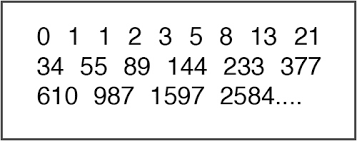
\includegraphics[width=80mm]{./imagenes/fibo.png}\\
		Figura 1
	\end{center}
	\bigskip
	Esto debido a que consiste en tomar 2 enteros proximos entre si e ir sumando el resultado con el contiguo predecesor del resultado, nuestro algoritmo recibe n que es el numero de los 
	primeros n dijitos de la sucesion que deseamos ver o calcular.
	\bigskip

	El siguiente algoritmo nos habla de la suma de los primeros n numeros naturales en su potencia cubica, de manera iterativa y recursiva, nuestro codigo pide un numero n que sera el numero de elementos tomados en la suma.
	
\newpage	
\section{Experimentaci\'on y Resultados}
	\subsection{Fibonacci}
	\subsubsection{Pseudocódigo de Fibonacci Recursivo}
	fiboRecu(n):\\
	Entrada: un entero positivo n\\
	Salida: El numero de la serie de Fibonacci con la posicion n \\
	1.- if n==1 or n==2:\\
	2.- \hspace{0.7cm}return 1\\
	3.- else:\\
	4.-  \hspace{0.7cm}return fiboRecu(n-1) + fiboRecu(n-2)\\	


	\subsubsection{Pseudocódigo de Fibonacci Iterativo}
	fiboIteracion(n):\\
	Entrada: un entero positivo n\\
	Salida: El numero de la serie de Fibonacci con la posicion n \\
	1.- a $\leftarrow$ 1\\
	2.-b $\leftarrow$ 1\\
	3.-for i=0 to i<n do:\\
	4.- \hspace{0.7cm}a $\leftarrow$ b \\
	5.- \hspace{0.7cm}b$\leftarrow$ a + b \\
	6.-return a
	
	{\large {\bf ii)Demostrar de manera formal que el algoritmo de fibonacci iterativo tiene orden lineal.}}\\
	fiboIteracion(n)  \hspace{4cm} Costo \hspace{4cm} Pasos\\
	1.- a $\leftarrow$ 1 \hspace{5cm} C1 \hspace{5cm} 1 \\
	2.- b $\leftarrow$ 1\hspace{5.1cm} C2 \hspace{5cm} 1 \\
	3.- for i=0 to i$<$n do:\hspace{3.3cm} C3 \hspace{5cm} n \\
	4.- \hspace{0.7cm}a $\leftarrow$ b  \hspace{4.3cm} C4 \hspace{5cm} n-1 \\
	5.- \hspace{0.7cm}b$\leftarrow$ a + b  \hspace{3.8cm} C5 \hspace{5cm} n-1 \\
	6.- return a\hspace{4.9cm} C6 \hspace{5cm} 1 \\\\
	{\bf ii)Demostracion.}
	Tenemos que:\\
	T(n) = C1 + C2 + C3n + C4(n-1) + C5(n-1) + C6\\
`	T(n) = C1 + C2 + C3n +C4n -C4 + C5n - C5 + C6\\
	Al factorizar nos queda:\\
	T(n) = (C3+C4+C5)n + (C1+C2-C4-C5+C6)\\
	$\therefore$\\
	T(n) $\in$ $\theta$(n)\\
\newpage
	{\large{\bf Mostrar con graficas que la proposicion anterior es cierta.}}\\
	Tomando valores desde 1 a 20 nos da:
	\begin{center}
				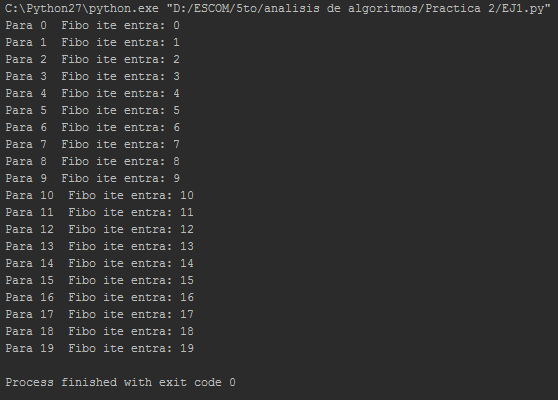
\includegraphics{./imagenes/fiboite1.png}\\
		Figura 2\\
	\end{center}
	\newpage
	La grafica para esta tabla es:\\
	\begin{center}
		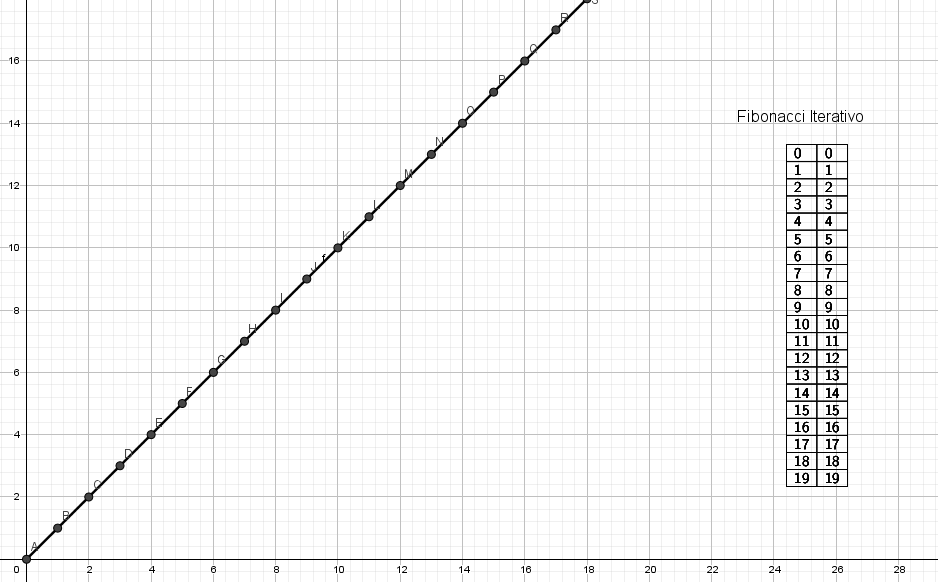
\includegraphics{./imagenes/fibo1.png}\\
		Figura 3\\
	\end{center}
	Podemos observar que la grafica para los valores obtenidos en la ejecucion del algoritmo muestra un comportamiento lineal, por lo 	el resultado tras la ejecucion, apoya la demostracion anterior
\newpage
	{\large{\bf A partir de graficas, proponer el orden de complejidad para el algoritmo recursivo.}}\\

	Tomando valores desde 1 a 20 nos da:
	\begin{center}
				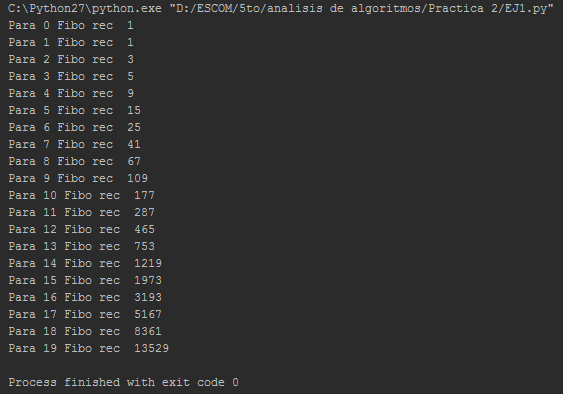
\includegraphics{./imagenes/fiborecu1.png}\\
		Figura 3\\
	\end{center}
	\newpage
	La grafica para esta tabla es:\\
	\begin{center}
		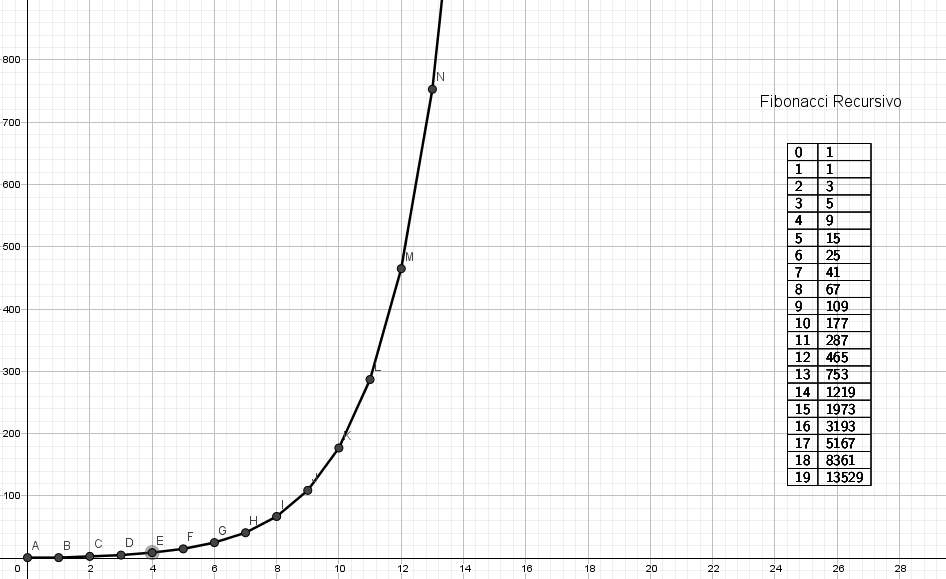
\includegraphics{./imagenes/fiborecu2.png}\\
		Figura 4\\
	\end{center}
	La grafica que nos arrojan los resultados obtenmidos en los experimentros es de tipo exponencial, por lo que se podria proponer O($n^{2}$)
	\subsection{Suma Cubica}
	\subsubsection{Apartir de graficas proponga una funcion g(n) tal que T(n) $\in$ O(g(n)) con T(n) como el tiempo computacional del algoritmo }
Para los valores del 1 al 50, el algoritmo arrojo los siguientes resultados:\\
\begin{center}
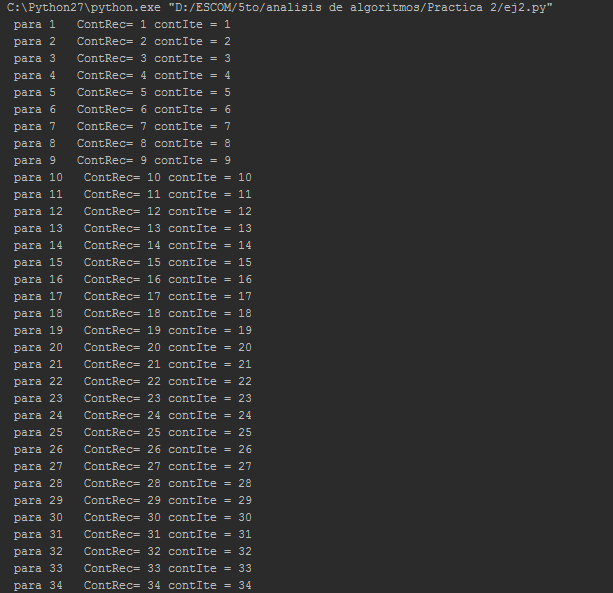
\includegraphics{./imagenes/suma1.png}\\
		Figura 5\\
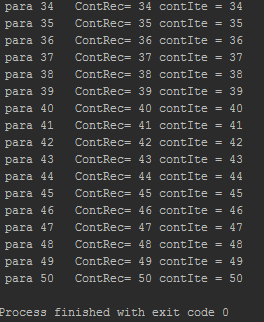
\includegraphics{./imagenes/suma2.png}\\
		Figura 6\\
	\end{center}
\newpage
La grafica, en ambos casos, da lo siguiente:\\
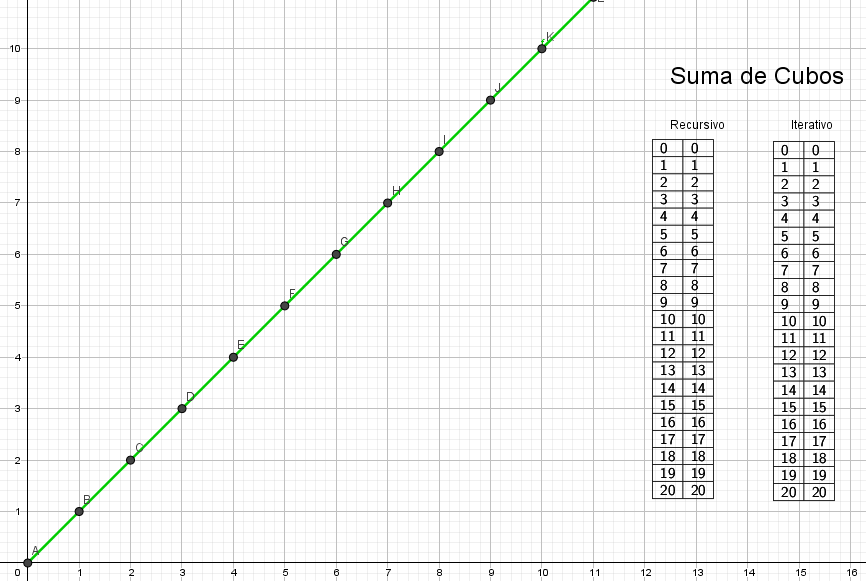
\includegraphics{./imagenes/graficaCubos.PNG}\\
\newpage
{\large{\bf-iii)Calcule el tiempo computacional del algoritmo recursivo e iterativo de manera formal. Compare sus resultados}}\\

	\bigskip
	
	{\bf{Forma Recursiva:}}
	
	\bigskip

	Sea A(n) el número de sumas que se realizan para calcular 	S(n). Entonces:

	\bigskip
	
	A(n) = 

	\bigskip

	Luego

	\bigskip

	A(n) = A(n-1) + 1

	\bigskip

	A(n) = A(n-2) + 1 + 1 = A(n-2) + 2

	\bigskip

	A(n) = A(n-3) + 1 + 2 = A(n-3) + 3

	\bigskip

	...
	
	\bigskip

	A(n) = A(n - (n - 1)) + n -1 = A(1) + n -1



	A(n) = 1+ n -1

	\bigskip

	A(n) = n

	\bigskip

	$\therefore$
	$ T(n) \quad\in\quad \theta(n)$	

	\bigskip

	{\bf{Forma Iterativa:}}

	\bigskip

	{\bf Algoritmo S(n)} \hspace{40mm}Costo \hspace{12mm} \#Pasos \\
	1.- \hspace{0.7cm}y $\leftarrow$ 0 \hspace{5.6cm} A \hspace{2.0cm} 1\\
	2.- \hspace{0.7cm}while n $\gtrdot$ 0 $\leftarrow$ 1 \hspace{4.0cm} B \hspace{2.0cm} n + 1\\
	3.-	\hspace{0.7cm}y $\leftarrow$ suma y  con x*x*x \hspace{3.0cm} C \hspace{2.0cm} n \\
	4.-	\hspace{0.7cm}n $\leftarrow$ n - 1 \hspace{5.0cm} D \hspace{2.0cm} n \\
	5.- \hspace{0.7cm}return y \hspace{5.3cm} E \hspace{2.0cm} 1 \\
	\bigskip

	Con ello tenemos que:

	T(n) = A + B(n + 1) + Cn + Dn + E
	\bigskip
	
	T(n) = (B + C + D)n + (A + B + E)
	\bigskip

	$\therefore$
	$ T(n) \quad\in\quad \theta(n)$		

	\bigskip

	\newpage

	\bigskip

	

	{	\newpage
	\section{Conclusi\'on General}
	En esta practica pudimos analizar 2 algoritmos basicos en la programacion, esto con 2 posibles maneras de ser resultos esto es de manera iterativa y recursiva, en mi trayectoria axademica claro que habia desarrollado estos algoritmos de ambas formas
pero nunca pense en cual podria sernos mas util o digamoslo asi computablemente viable, es por esto que para empezar me gustaria hablar del algoritmo de Fibonacci de este ser podia intuir un poco que el algoritmo iterativo nos seria mas
conveniente, ya que la recursividad es conocida por ser un arma de doble filo, es poderosa cuando se sabe ocupar y detener, pero el algoritmo de la suma de los cubos me fue algo extraño de aceptar ya que los datos y las graficas no eran lo que esperaba,
lo que mas ocupo mi trabajo en definitiva fue analizar los resultados ya que requerian de mas atencion que programar o graficar, pero convenientemente los resultados fueron satisfactorios y a mi consideracion de hoy en adelante seria de
gran ayuda para cualquier programador un aviso cuando tengamos que programar Fibonacci nos recuerde o nos avise que es mejor programar este de manera iterativa.
	\newpage
	\section{Anexos}
	
	{\Large{\bf Algoritmo Bubble-Sort}}\\
	Sea A.largo = n \\
	BubbleSort(A)	 \hspace{6cm}  Costo	 \hspace{2.5cm} 						Pasos \\
1.- \hspace{0.7cm}		for i=1 to A.largo -1 do			 \hspace{3.2cm}C1	\hspace{3cm}n \\
2.- \hspace{0.7cm}			for j= A.largo downto i+1		 \hspace{2.8cm}C2	\hspace{3cm}$\sum_{i=1}^{n-1} t_i$	\\
3.- \hspace{0.7cm} \hspace{0.7cm}				if A[j] < A[j-1] \hspace{4cm}C3	\hspace{3cm} $\sum_{i=1}^{n-1} (t_i-1)$\\
4.- \hspace{0.7cm} \hspace{0.7cm} \hspace{0.7cm}					exchange(A[j], A[j-1]	 \hspace{2cm}C4	\hspace{3cm}$\sum_{i=1}^{n-1} R_i$\\
\\
El Peor de los casos se presenta cuando el arreglo esta ordenado en forma decreciente, por lo que: \\
Para \(i = 1,       t_1 =n\)	\\
Para \(i = 2, t_2 =n-1\)	\\
Para \(i = 3, t_3 =n-3\)	\\
.\\
.\\
.\\
Para \(i = k,    t_k =n-k+1\)	\\
Así  \(t_i =n-i+1\)	\\
Y  \(R_i = t_i -1\)	\\
Con ello, tenemos que:\\
\\
T(n) = C1n + C2($\sum_{i=1}^{n-1}( n-i+1($) + C3($ \sum_{i=1}^{n-1} (n-i) $) + C4($sum_{i=1}^{n-1}( n-i)$)\\
T(n) = C1n + C2n($\sum_{i=1}^{n-1} n$) - C2($\sum_{i=1}^{n-1} i $)  + C2($\sum_{i=1}^{n-1} i $) - C3($\sum_{i=1}^{n-1} n $) -C3($\sum_{i=1}^{n-1} i $) + C4($\sum_{i=1}^{n-1} n $) - C4($\sum_{i=1}^{n-1} i $)\\
\\ 
T(n) = C1n + (C2+C3+C4)($\sum_{i=1}^{n-1} n$) - (C2+C3+C4)($\sum_{i=1}^{n-1} i$) + C2(n-1) \\
T(n) = C1n + (C2+C3+C4)(n(n-1)) - (C2+C3+C4)($\dfrac{n(n+1)}{2}$) + C2(n-1) \\
T(n) = (C1 + $\dfrac{C2+C3+C4}{2}$)n + ($\dfrac{C2+C3+C4}{2}$)$n^{2}$ \\
Por lo tanto, tenemos:\\
T(n) $\in$ O($n^{2}$)

El mejor de los casos se da cuando el arreglo ya esta ordenado de forma creciente.\\
En dicho caso, lo unico que hay que cambiar es la condicion del if, ya que nunca se cumple, por lo tanto: \\
$R_i = 0$ \\
Por lo tanto:  \\
T(n) = C1n + C2($\sum_{i=1}^{n-1}( n-i+1)$) + C3($\sum_{i=1}^{n-1}( n-i)$) \\
T(n) = (C1+$\dfrac{C2+C3}{2}$)n + ($\dfrac{C2+C3}{2}$)$n^{2}$ \\
$\therefore$ \\
T(n) $\in$ $\Omega$($n^{2}$) \\
$\therefore$\\
T(n) $\in$ $\theta$($n^{2}$) \\

	\bigskip	
	
	\section{Bibliografía}
	\begin{itemize}
		\item Brassard, G. (1997). Fundamentos de Algoritmia. España: Ed. Prentice Hall. ISBN 		848966000X
		\item Harel, D. (2004). Algorithmics: The spirit of Computing (3rd. Ed). Estados Unidos de América: Addison
Wesley. ISBN-13: 978-0321117847
	\end{itemize}
	

\end{document}